\section{Algorytm \textit{ALERGIA}}  
\label{sec:alergia}  

Algorytm \textit{ALERGIA} \cite{ALERGIA} jest stosowany do indukcji stochastycznych gramatyk regularnych. W przeciwieństwie do \textit{RPNI} lub \textit{GIG}, które zakładają obecność zarówno przykładów pozytywnych, jak i negatywnych, \textit{ALERGIA} opiera się wyłącznie na zbiorze przykładów pozytywnych. Umożliwia to jego zastosowanie w sytuacjach, gdzie dostęp do przykładów negatywnych jest ograniczony lub niemożliwy.  

Algorytm ten konstruuje deterministyczny stochastyczny automat skończony (DSFA) na podstawie drzewa akceptacji prefiksów (PTA) utworzonego z dostępnych danych. Proces uogólniania polega na łączeniu stanów automatu, przy jednoczesnym zachowaniu zgodności ze statystycznym rozkładem prawdopodobieństwa przejść między stanami. Decyzje o scalaniu są podejmowane na podstawie testów statystycznych, które zapewniają, że wynikowy model zachowuje probabilistyczne własności danych wejściowych.  

Jedną z kluczowych cech algorytmu \textit{ALERGIA} jest jego zdolność do indukcji gramatyk stochastycznych, co czyni go szczególnie przydatnym w zastosowaniach wymagających modelowania niepewności lub probabilistycznych wzorców zachowań. Dzięki swojej efektywności obliczeniowej algorytm ten znajduje zastosowanie w zadaniach takich jak rozpoznawanie wzorców, analiza sekwencji biologicznych oraz modelowanie języka naturalnego.

Algorytm działa iteracyjnie, testując kompatybilność stanów i łącząc te, które są statystycznie zgodne. Proces kończy się, gdy żadne dalsze scalenie nie jest możliwe bez naruszenia kryteriów statystycznych. Dzięki temu wynikowy automat nie tylko reprezentuje język generowany przez dane treningowe, ale także umożliwia estymację prawdopodobieństwa generacji nowych ciągów.


\subsection{Metoda}  
Algorytm \textit{ALERGIA} pozwala na indukcję deterministycznego stochastycznego automatu skończonego (DSFA), który przybliża rozkład prawdopodobieństwa nad danymi wejściowymi. Proces ten obejmuje następujące kroki:  

\paragraph*{Opis algorytmu.}  
Algorytm \textit{ALERGIA} składa się z kilku etapów:  
\begin{enumerate}  
    \item \textbf{Budowa drzewa prefiksów (PTA):}  
        Zbiór przykładów pozytywnych jest używany do zbudowania deterministycznego automatu reprezentującego dokładnie wszystkie sekwencje w danych.  
    \item \textbf{Iteracyjne łączenie stanów:}  
        Algorytm analizuje pary stanów w PTA i testuje ich zgodność statystyczną. Łączenie stanów jest realizowane tylko wtedy, gdy nie narusza statystycznej zgodności z danymi.  
    \item \textbf{Sprawdzanie zgodności:}  
        Kompatybilność stanów jest oceniana za pomocą testu Hoeffding'a oraz dodatkowego testu dla rozkładów wykładniczych czasów przejść.  
    \item \textbf{Zakończenie:}  
        Algorytm kończy działanie, gdy żadne dalsze scalenie stanów nie jest możliwe bez naruszenia zgodności statystycznej. Ostateczny automat aproksymuje rozkład probabilistyczny danych wejściowych.  
\end{enumerate}


\subsection{Formalizacja}  
W tej sekcji przedstawiono matematyczne podstawy algorytmu \textit{ALERGIA} oraz definicje kluczowych pojęć, które umożliwiają precyzyjne opisanie jego działania. Algorytm ten wykorzystuje akceptor drzewa prefiksów (PTA) jako strukturę początkową z definicji \ref{def:pta}. Proces formalizacji skupia się na mechanizmach scalania stanów, które pozwalają na stopniowe upraszczanie automatu przy jednoczesnym zachowaniu zgodności z probabilistycznymi wzorcami danych wejściowych.  

\begin{definition}[DSFA]  
\label{def:dsfa}
Stochastyczny, skończony automat deterministyczny to piątka uporządkowana
\[ 
A = (Q, \Sigma, \delta, q_0, P), 
\]
gdzie:  
\begin{itemize}  
    \item \( Q \) – skończony zbiór stanów,  
    \item \( \Sigma \) – alfabet,  
    \item \( \delta : Q \times \Sigma \to Q \) – funkcja przejścia,  
    \item \( q_0 \in Q \) – stan początkowy,  
    \item \( P: Q \times \Sigma \to [0, 1] \) – funkcja prawdopodobieństwa przejść, spełniająca:  
    \[
    \sum_{a \in \Sigma} P(q, a) \leq 1, \quad \forall q \in Q, \quad a \in \Sigma.
    \]  
\end{itemize}
\end{definition}

Automat \( A \) generuje język stochastyczny, w którym każda sekwencja symboli z \( \Sigma \) jest akceptowana z określonym prawdopodobieństwem, wyznaczanym przez funkcję \( P \).

\begin{definition}[Zgodność stanów]  
\label{def:alergia_state_compatibility}
Dwa stany \( q_1, q_2 \in Q \) są uznawane za zgodne (kompatybilne) i mogą zostać scalone, jeżeli spełnione są dwa warunki:  
\begin{enumerate}
    \item Funkcja prawdopodobieństwa przejść \( P \) dla każdego symbolu \( a \in \Sigma \) spełniają:  
    \[
    |P(q_1, a) - P(q_2, a)| \leq \epsilon,
    \]  
    gdzie \( \epsilon \) jest granicą wyznaczoną przez test Hoeffding’a:  
    \[
    \epsilon = \sqrt{\frac{1}{2} \ln\left(\frac{2}{\alpha}\right)} \left( \frac{1}{\sqrt{n_1}} + \frac{1}{\sqrt{n_2}} \right),
    \]  
    przy czym:  
    \begin{itemize}  
        \item \( n_1 \) – liczba obserwacji dla stanu \( q_1 \),  
        \item \( n_2 \) – liczba obserwacji dla stanu \( q_2 \),  
        \item \( \alpha \) – poziom ufności.  
    \end{itemize}
    \item Prawdopodobieństwa terminacji \( F \) spełniają:
    \[
    |F(q_1) - F(q_2)| \leq \epsilon,
    \]  
\end{enumerate}
\end{definition}

Test Hoeffding’a to statystyczna metoda oceny zgodności dwóch rozkładów prawdopodobieństwa, bazująca na nierówności Hoeffding’a. W kontekście algorytmu \textit{ALERGIA} test ten służy do sprawdzania, czy różnice między obserwowanymi częstościami przejść w stanach automatu można uznać za przypadkowe, czy też są one statystycznie istotne.  

Nierówność Hoeffding’a zapewnia górne ograniczenie na prawdopodobieństwo, że rzeczywiste wartości oczekiwane dwóch zmiennych losowych odbiegają od ich wartości estymowanych o więcej niż zadana tolerancja \( \epsilon \). 

W algorytmie \textit{ALERGIA} test Hoeffding’a porównuje rozkłady przejść pomiędzy stanami automatu. Jeśli różnice są mniejsze niż wyznaczony próg tolerancji, stany są uznawane za zgodne statystycznie i mogą zostać scalone.  

\begin{definition}[Łączenie stanów w \textit{ALERGIA}]  
\label{def:alergia_state_merging}  
Łączenie dwóch stanów \( q_1, q_2 \in Q \) w stochastycznym, skończonym automacie deterministycznym (DSFA) \( A = (Q, \Sigma, \delta, q_0, P) \) polega na utworzeniu nowego automatu \( A' = (Q', \Sigma, \delta', q_0, P') \), gdzie stan \( q_1 \) reprezentuje połączone stany, a \( q_2 \) zostaje usunięty. Funkcje przejścia i prawdopodobieństwa są aktualizowane zgodnie z poniższymi regułami:  
\begin{itemize}  
    \item \( Q' = Q \setminus \{q_2\} \),  
    \item \( \delta'(q, a) =  
    \begin{cases}  
        \delta(q_1, a) & \text{jeśli } \delta(q, a) = q_2, \\  
        \delta(q, a) & \text{w przeciwnym przypadku.}  
    \end{cases}  
    \)  
    \item Prawdopodobieństwa przejść są uśredniane w następujący sposób:  
    \[
    P'(q, a) = \frac{n_1 \cdot P(q_1, a) + n_2 \cdot P(q_2, a)}{n_1 + n_2},
    \]  
    gdzie \( n_1 \) i \( n_2 \) to liczby obserwacji w stanach \( q_1 \) i \( q_2 \).  
\end{itemize}  
\end{definition}  

Łączenie stanów jest przeprowadzane tylko wtedy, gdy dwa stany są zgodne według definicji \ref{def:alergia_state_compatibility}. Po scaleniu stanów \( q_1 \) i \( q_2 \) nowy stan dziedziczy przejścia oraz rozkłady prawdopodobieństwa jako uśrednienie. Scalanie w algorytmie kończy się, gdy żadne dalsze połączenia nie spełniają powyższych kryteriów zgodności.


\subsection{Złożoność}  
Algorytm \textit{ALERGIA} cechuje się złożonością wielomianową, zależną od rozmiaru danych wejściowych. W analizie złożoności czasowej i pamięciowej uwzględniamy następujące parametry:  
\begin{itemize}  
    \item \(|S^+|\) - liczba przykładów pozytywnych,  
    \item \( l^+ \) - maksymalna długość ciągu w \( S^+ \),  
    \item \(|\Sigma|\) - liczba symboli w alfabecie.  
\end{itemize}  

\paragraph*{Złożoność czasowa}  
Algorytm \textit{ALERGIA} składa się z dwóch głównych etapów:  
\begin{enumerate}  
    \item \textbf{Budowa drzewa prefiksowego (PTA):}  
    Tworzenie drzewa wymaga przetworzenia wszystkich słów w zbiorze \( S^+ \), analizując je symbol po symbolu. Koszt tego kroku wynosi:  
    \[
    O(|S^+| \cdot l^+).
    \]  

    \item \textbf{Scalanie stanów:}  
    Każda para stanów w PTA jest analizowana pod kątem zgodności. Liczba stanów wynosi \( O(|S^+| \cdot l^+) \), co prowadzi do \( O((|S^+| \cdot l^+)^2) \) możliwych par do porównania.  

    Ponadto, dla każdej pary stanów sprawdzana jest zgodność ich rozkładów prawdopodobieństwa, co wymaga przeprowadzenia testów statystycznych (np. testu Hoeffding’a) dla wszystkich symboli w alfabecie \( \Sigma \). Złożoność tego kroku wynosi:  
    \[
    O(|\Sigma|).
    \]
\end{enumerate}  

\paragraph*{Łączna złożoność czasowa}  
Po uwzględnieniu obu etapów oraz kosztów związanych z rekurencyjnym sprawdzaniem zgodności, całkowita złożoność czasowa algorytmu \textit{ALERGIA} w najgorszym przypadku wynosi:  
\[
O((|S^+| \cdot l^+)^2 \cdot |\Sigma|).
\]

\paragraph*{Złożoność pamięciowa}  
Algorytm przechowuje następujące struktury:  
\begin{itemize}  
    \item \textbf{Drzewo prefiksowe (PTA):}  
    PTA składa się z \( O(|S^+| \cdot l^+) \) stanów, z których każdy może mieć do \( |\Sigma| \) przejść. Wymagana przestrzeń pamięci wynosi:  
    \[
    O(|S^+| \cdot l^+ \cdot |\Sigma|).
    \]  

    \item \textbf{Statystyki przejść:}  
    Dla każdego stanu przechowywane są rozkłady prawdopodobieństw oraz dane statystyczne, co daje dodatkowy koszt pamięciowy:  
    \[
    O(|S^+| \cdot l^+).
    \]  
\end{itemize}  

Łączna złożoność pamięciowa wynosi:  
\[
O(|S^+| \cdot l^+ \cdot |\Sigma|).
\]  

\paragraph*{Czynniki wpływające na złożoność}  
Efektywność algorytmu \textit{ALERGIA} zależy przede wszystkim od liczby przykładów pozytywnych (\( S^+ \)) oraz długości słów (\( l^+ \)), które determinują rozmiar drzewa prefiksowego i liczbę stanów do analizy. Dodatkowo, większy alfabet (\( |\Sigma| \)) zwiększa liczbę możliwych przejść, co wpływa zarówno na czas obliczeń, jak i wymagania pamięciowe. 

\subsection{Przykład działania}  
Aby zilustrować działanie algorytmu \textit{ALERGIA}, rozważmy prosty przykład danych wejściowych opisujących sekwencje wyników rzutów monetą. Każdy wynik jest oznaczony symbolem \( H \) (orzeł) lub \( T \) (reszka).

\paragraph*{Dane wejściowe.}  
Zbiór przykładów pozytywnych (\( S^+ \)):  
\[
S^+ = \{H, H, T, HH, HT, TH, TT, HHH\}.
\]  

\paragraph*{Krok 1: Konstrukcja drzewa prefiksowego (PTA).}  
Na podstawie danych pozytywnych algorytm buduje drzewo prefiksowe (Prefix Tree Acceptor, PTA), które reprezentuje dokładnie wszystkie obserwowane sekwencje. Każdy stan odpowiada prefiksowi słów z \( S^+ \), a przejścia są etykietowane symbolami \( H \) lub \( T \). Wynik tego kroku można zobaczyć na rysunku \ref{fig:alergia_example_0}. 

\begin{figure}[ht]
    \centering
    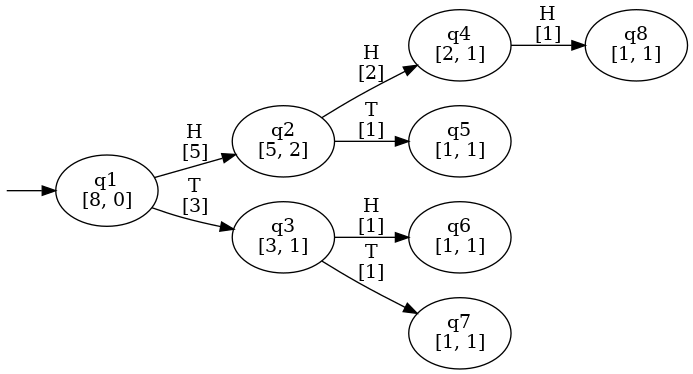
\includegraphics[width=0.8\textwidth]{images/run_example/alergia/0.png}
    \caption{Drzewo prefiksowe (PTA) skonstruowane dla \( S^+ \).}
    \label{fig:alergia_example_0}
\end{figure}

\paragraph*{Krok 2: Scalanie stanów \( q_1 \) i \( q_2 \).}  
Algorytm rozpoczyna proces scalania stanów od analizy zgodności pierwszej pary stanów \( q_1 \) i \( q_2 \). Weryfikacja odbywa się na podstawie rozkładów prawdopodobieństw przejść oraz liczby zakończeń w obu stanach.  

\paragraph*{Dane stanów:}  
\begin{itemize}  
    \item \( q_1 \): \( n = 8, F = 0 \), przejścia: \( H[5], T[3] \).  
    \item \( q_2 \): \( n = 5, F = 2 \), przejścia: \( H[2], T[1] \).  
\end{itemize}  

\paragraph*{Sprawdzenie terminacji:}  
Prawdopodobieństwo terminacji dla każdego stanu:  
\[
P_F(q_1) = \frac{0}{8} = 0, \quad P_F(q_2) = \frac{2}{5} = 0.4.
\]

Różnica:  
\[
|P_F(q_1) - P_F(q_2)| = |0 - 0.4| = 0.4.
\]

\paragraph*{Tolerancja Hoeffding’a:}  
Przy poziomie ufności \( \alpha = 1.25 \) oraz liczbach obserwacji \( n_1 = 8 \) i \( n_2 = 5 \), granica zgodności \( \epsilon \) jest obliczana na podstawie wzoru:  
\[
\epsilon = \sqrt{\frac{\ln(2 / \alpha)}{2}} \left( \frac{1}{\sqrt{n_1}} + \frac{1}{\sqrt{n_2}} \right).
\]

\paragraph*{Podstawienie wartości:}  
\[
\epsilon = \sqrt{\frac{\ln(2 / 1.25)}{2}} \left( \frac{1}{\sqrt{8}} + \frac{1}{\sqrt{5}} \right).
\]

Najpierw obliczamy logarytm:  
\[
\ln\left(\frac{2}{1.25}\right) = \ln(1.6) \approx 0.470.
\]

Podstawiamy:  
\[
\epsilon = \sqrt{\frac{0.470}{2}} \left( \frac{1}{\sqrt{8}} + \frac{1}{\sqrt{5}} \right).
\]

\[
\epsilon = \sqrt{0.235} \left( \frac{1}{2.828} + \frac{1}{2.236} \right).
\]

\[
\epsilon \approx 0.485 \left( 0.354 + 0.447 \right).
\]

\[
\epsilon \approx 0.485 \cdot 0.801 \approx 0.389.
\]

\paragraph*{Porównanie:}  
Ponieważ:  
\[
0.4 > 0.389,
\]  
stany \( q_1 \) i \( q_2 \) **nie mogą zostać połączone** bez dalszej analizy ich następców.  

\paragraph*{Rekurencyjna zgodność:}  
Aby kontynuować proces, algorytm przeprowadza sprawdzanie zgodności dla następujących par stanów:  
\begin{itemize}  
    \item \( q_1 \to q_3 \) i \( q_2 \to q_5 \).  
    \item \( q_2 \to q_4 \) i \( q_4 \to q_8 \).  
\end{itemize}  

Po dodatkowej analizie Hoeffding’a, wszystkie pary okazują się zgodne, co umożliwia scalanie całych podstruktur.  

\paragraph*{Rekurencyjne sprawdzanie następników:}  
Aby kontynuować analizę, algorytm porównuje następujące pary stanów:  
\begin{itemize}  
    \item \( q_1 \to q_3 \) i \( q_2 \to q_5 \).  
    \item \( q_2 \to q_4 \) i \( q_4 \to q_8 \).  
\end{itemize}  

Na podstawie testu Hoeffding’a wszystkie te pary okazują się zgodne, co pozwala na scalanie całych podstruktur.  

\paragraph*{Wynik:}  
Po scaleniu stanów \( q_1, q_2, q_4, q_8 \) oraz \( q_3, q_5 \) powstają dwa nowe stany:  
\begin{itemize}  
    \item \( q_1 \): \( n = 16, F = 4 \), przejścia: \( H[8], T[4] \).  
    \item \( q_3 \): \( n = 4, F = 2 \), przejścia: \( H[1], T[1] \).  
\end{itemize}  

Wynik tego kroku przedstawiono na rysunku \ref{fig:alergia_example_1}.  

\begin{figure}[ht]
    \centering
    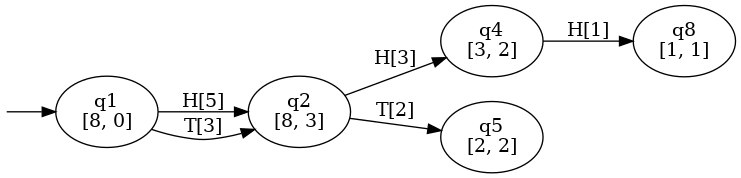
\includegraphics[width=0.8\textwidth]{images/run_example/alergia/1.png}
    \caption{Graf po scaleniu stanów \( q_1, q_2, q_4, q_8 \) oraz \( q_3, q_5 \).}
    \label{fig:alergia_example_1}
\end{figure}  
